\chapter{Operationalization}

\section*{Why This Matters}

Production deployment represents only the beginning of a model's operational lifecycle. Models require ongoing management, monitoring, and maintenance to sustain performance and deliver business value. Unlike traditional software, which remains stable once deployed, machine learning models degrade over time as production data distributions shift, requiring systematic retraining, version management, and continuous evaluation.

The operational phase typically accounts for 60-80\% of total AI system costs over a three-year horizon. Training a model might cost \$50,000, but operating it—serving predictions, monitoring performance, retraining periodically, managing versions, and maintaining infrastructure—costs \$150,000-\$400,000 annually. Understanding these operational requirements is essential for realistic budget planning, infrastructure sizing, and organizational capability assessment.

This chapter examines the technical and economic factors governing production AI operations, covering model lifecycle management, continuous training strategies, security considerations, and cost optimization approaches. The focus is on building sustainable operational practices that maintain model performance while controlling costs.

\section{Model Lifecycle Management}

Production models progress through distinct lifecycle stages, each with specific technical requirements and operational characteristics. Managing this lifecycle effectively requires version control systems, deployment strategies, and rollback capabilities comparable to traditional software engineering, but adapted for the unique characteristics of machine learning systems.

\subsection{Lifecycle Stages}

Models transition through research, staging, and production environments, with each stage serving specific validation purposes. The research environment supports experimentation and initial development, typically using smaller datasets and less expensive hardware. Models in research undergo rapid iteration, with dozens or hundreds of training runs exploring architectural variations, hyperparameter settings, and data preprocessing approaches. Infrastructure costs remain modest—perhaps \$5,000-\$20,000 monthly for a team of 5-10 researchers using shared GPU clusters.

The staging environment replicates production conditions for final validation before deployment. Staging uses production-scale data, production-equivalent hardware, and production API interfaces. This environment validates performance under realistic conditions, tests integration with downstream systems, and measures actual latency and throughput. Staging infrastructure typically mirrors production at 10-20\% scale, sufficient for load testing and integration validation without full production costs. For a production system serving 1,000 requests per second, staging might handle 100-200 requests per second, costing \$10,000-\$30,000 monthly.

Production represents the operational environment serving live traffic. Production infrastructure must provide the reliability, performance, and scalability required for business operations. This includes redundancy for high availability, monitoring for performance tracking, and capacity for peak load handling. Production costs scale with traffic volume and latency requirements. A system serving 1,000 requests per second with 100ms latency requirements might cost \$50,000-\$150,000 monthly, depending on model size and optimization level.

\subsection{Version Management}

Model versioning requires tracking not just model weights, but the complete artifact set necessary for reproducible deployment: training code, data preprocessing pipelines, hyperparameter configurations, dependency versions, and evaluation metrics. Unlike code versioning, which tracks text files, model versioning handles multi-gigabyte binary artifacts and complex dependency graphs.

A comprehensive version management system tracks model artifacts with unique identifiers linking to specific training runs. For a BERT-base model, this includes the 440 MB model checkpoint, the tokenizer vocabulary and configuration, the preprocessing pipeline code, the training dataset version or hash, the hyperparameter configuration, and the evaluation metrics on validation and test sets. Storage costs accumulate quickly: maintaining 50 model versions at 500 MB each consumes 25 GB, costing approximately \$0.60 monthly on S3 standard storage, but potentially \$25-\$50 monthly when including associated metadata, logs, and evaluation artifacts.

Version metadata enables critical operational capabilities. Each version records training date, training duration and cost, dataset version, evaluation metrics across multiple test sets, deployment history, and performance monitoring data. This metadata supports impact analysis when issues arise, cost attribution for budget tracking, and compliance documentation for regulated industries.

\subsection{Deployment Patterns}

Production deployment strategies balance risk mitigation against operational complexity. Three primary patterns—blue-green deployment, canary deployment, and shadow deployment—offer different trade-offs between safety, resource requirements, and validation thoroughness.

Blue-green deployment maintains two complete production environments, switching traffic between them atomically. The blue environment serves production traffic while the green environment receives the new model version. After validation in the green environment, traffic switches completely from blue to green. This approach provides instant rollback capability—simply switch traffic back to blue if issues arise—and zero-downtime deployment. However, it requires double the infrastructure capacity during deployment windows, increasing costs by 50-100\% during these periods. For a system normally costing \$100,000 monthly, blue-green deployment adds \$50,000-\$100,000 in temporary infrastructure costs per deployment.

Canary deployment gradually shifts traffic to the new model version, starting with a small percentage and increasing as confidence grows. Initial deployment might route 1\% of traffic to the new version, increasing to 5\%, 10\%, 25\%, 50\%, and finally 100\% over hours or days. This approach limits blast radius—if the new version performs poorly, only a small fraction of users are affected—and provides real-world validation before full deployment. Canary deployment requires sophisticated traffic routing and monitoring infrastructure, but adds minimal infrastructure costs beyond the new model version's serving capacity.

Shadow deployment runs the new model version in parallel with the current production version, logging predictions without serving them to users. This approach enables thorough validation with zero user impact, comparing new and old model predictions on real production traffic. Shadow deployment requires additional serving capacity equal to the new model's requirements—effectively doubling inference costs during the shadow period—but provides the highest confidence validation. For critical systems where deployment failures carry significant business risk, the additional cost of shadow deployment often justifies the risk reduction.

\subsection{Rollback Strategies}

Effective rollback capabilities require maintaining previous model versions in deployable state and implementing automated rollback triggers. The previous production version should remain deployed and ready to receive traffic, enabling rollback within seconds or minutes rather than hours. This requires keeping the previous version's serving infrastructure active, adding 10-20\% to infrastructure costs but providing essential risk mitigation.

Automated rollback triggers monitor key performance indicators and revert to the previous version when degradation exceeds thresholds. Typical triggers include error rate increases beyond baseline, latency degradation beyond SLA requirements, prediction distribution shifts indicating model failure, and business metric degradation such as conversion rate drops. For a model normally maintaining 0.1\% error rate and 50ms p95 latency, rollback might trigger automatically if error rate exceeds 0.5\% or latency exceeds 100ms for more than 5 minutes.

\begin{figure}[htbp]
\centering
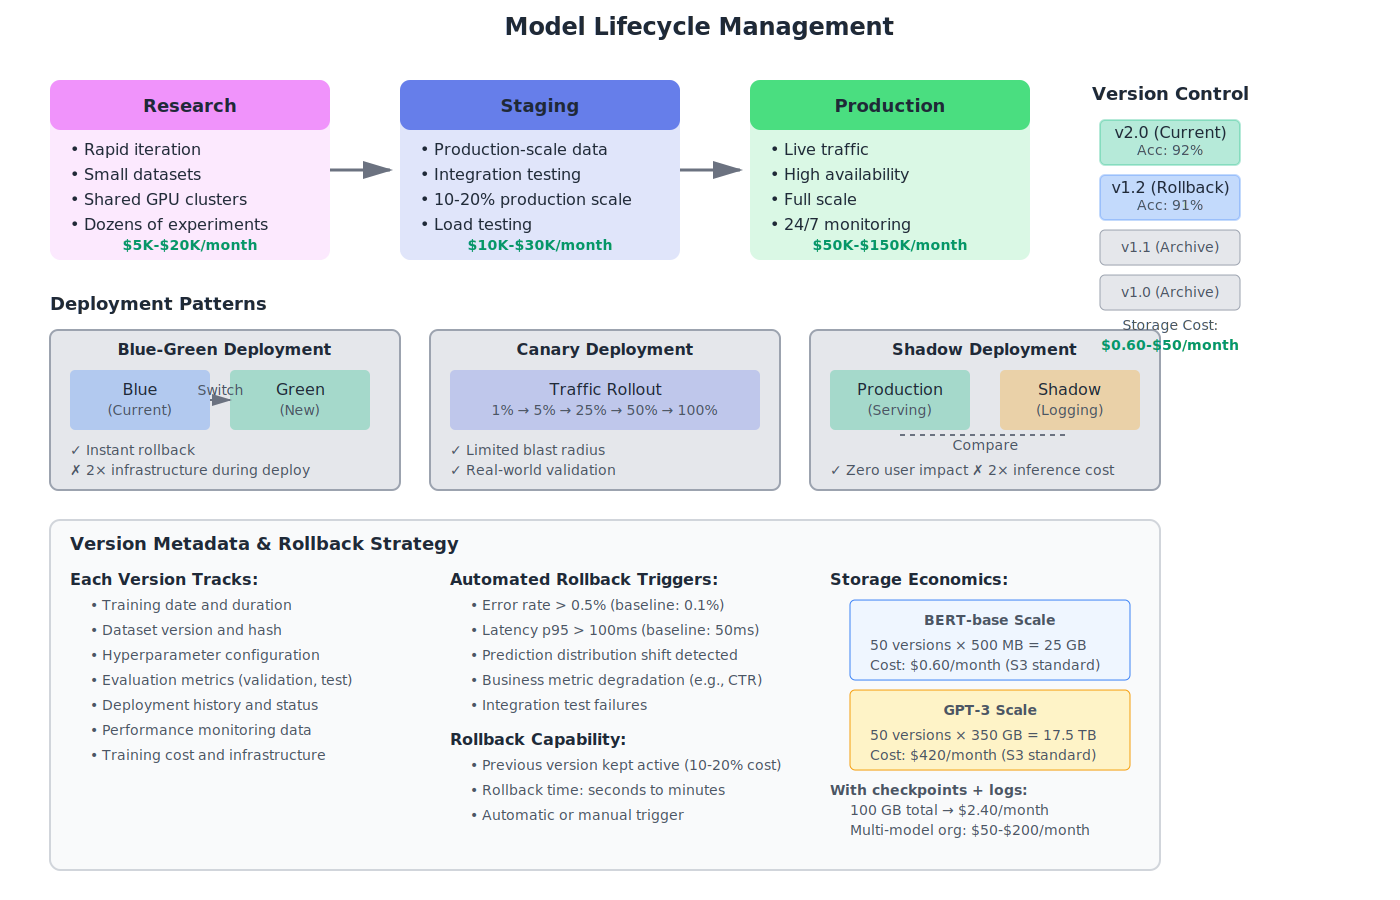
\includegraphics[width=0.95\textwidth]{chapters/diagrams/chapter09_lifecycle_q1r2s3t4.png}
\caption{Model lifecycle management showing progression from research through production environments, deployment patterns (blue-green, canary, shadow), version control strategy, and storage economics. Each environment stage has distinct characteristics and cost profiles, with production requiring the highest reliability and scale.}
\label{fig:lifecycle}
\end{figure}

\subsection{Storage Costs}

Model artifact storage costs scale with version retention policies and artifact sizes. A retention policy maintaining the current production version, the previous production version for rollback, the last 10 staging versions for analysis, and monthly snapshots for the past year generates specific storage requirements. For BERT-base models at 500 MB per version, this policy requires approximately 6 GB storage, costing \$0.15 monthly on S3 standard storage. For GPT-3 scale models at 350 GB per version, the same policy requires 4.2 TB, costing \$100 monthly.

Storage costs increase significantly when including training checkpoints, evaluation datasets, and experiment logs. A comprehensive artifact repository for a production model might include 50 model versions at 500 MB each (25 GB), 100 training checkpoints at 500 MB each (50 GB), evaluation datasets and results (10 GB), and training logs and metrics (15 GB), totaling 100 GB and costing \$2.40 monthly on S3 standard storage. For organizations managing dozens of production models, storage costs reach \$50-\$200 monthly, modest compared to training and serving costs but requiring management to prevent unbounded growth.

\section{Continuous Training and Evaluation}

Model performance degrades over time as production data distributions shift from training data distributions. This degradation, called model drift or concept drift, necessitates periodic retraining to maintain performance. Understanding when to retrain, how to automate the retraining process, and how to evaluate ongoing performance is essential for sustainable production operations.

\subsection{Model Drift and Retraining Triggers}

Model drift manifests as gradual performance degradation on production data. A sentiment analysis model trained on 2023 data might achieve 92\% accuracy initially, but degrade to 88\% accuracy after six months as language patterns evolve, new products and brands emerge, and cultural references shift. The degradation rate varies by domain: news and social media models drift rapidly (weeks to months), e-commerce and search models drift moderately (months to quarters), and medical and legal models drift slowly (quarters to years).

Retraining triggers should be based on measured performance degradation rather than fixed schedules. Continuous evaluation on held-out test sets or human-labeled production samples provides ongoing performance measurement. When performance drops below acceptable thresholds—for example, accuracy falling from 92\% to 89\%, or precision dropping from 85\% to 80\%—retraining becomes necessary. This approach ensures retraining occurs when needed rather than on arbitrary schedules, optimizing the trade-off between performance maintenance and retraining costs.

Data distribution shifts provide an earlier signal than performance degradation. Monitoring input feature distributions, prediction distributions, and confidence scores can detect drift before performance degrades significantly. For a model trained on data with mean feature values of 0.5 and standard deviation 0.2, production data showing mean 0.6 and standard deviation 0.3 indicates distribution shift likely to cause performance degradation. Triggering retraining based on distribution shift enables proactive maintenance before user-visible performance issues arise.

\subsection{Retraining Costs and Economics}

Retraining costs depend on model size, dataset size, and retraining frequency. For BERT-base trained on 10 million documents, retraining from scratch requires approximately 20 GPU-hours on A100 hardware, costing \$50-\$100 on cloud spot instances. Retraining quarterly costs \$200-\$400 annually. For larger models, costs scale proportionally: a GPT-3 scale model requiring 1,000 GPU-days for initial training might require 100-200 GPU-days for retraining on updated data, costing \$250,000-\$500,000 per retraining cycle.

Fine-tuning from the previous model version rather than training from scratch reduces costs significantly. Fine-tuning typically requires 10-20\% of full training time, as the model already captures general patterns and needs only to adapt to distribution shifts. For BERT-base, fine-tuning might require 2-4 GPU-hours, costing \$5-\$10. This 10× cost reduction makes more frequent retraining economically viable, enabling monthly or even weekly updates for rapidly drifting domains.

The economic trade-off balances retraining costs against performance degradation costs. If model accuracy degradation from 92\% to 89\% costs \$10,000 monthly in lost revenue or increased support costs, spending \$1,000 monthly on retraining provides strong ROI. Conversely, if performance degradation has minimal business impact, less frequent retraining makes economic sense. This calculation should drive retraining frequency decisions rather than arbitrary schedules.

\subsection{Continuous Evaluation Strategy}

Continuous evaluation requires ongoing measurement of model performance on production data. Three primary approaches—held-out test sets, human labeling of production samples, and proxy metrics—provide different trade-offs between cost, accuracy, and timeliness.

Held-out test sets provide consistent performance measurement over time. Maintaining a fixed test set of 10,000 labeled examples enables tracking performance trends as the model and production data evolve. However, held-out test sets become stale, eventually diverging from production data distribution and providing misleading performance estimates. Test set maintenance requires periodic updates with recent production data, necessitating human labeling costs.

Human labeling of production samples provides accurate performance measurement on current data. Randomly sampling 100-1,000 production examples weekly or monthly and obtaining human labels enables direct performance measurement. For a model serving 1 million predictions monthly, sampling 1,000 examples (0.1\%) and obtaining labels at \$0.50 per example costs \$500 monthly. This approach provides accurate, current performance measurement but requires ongoing labeling budget.

Proxy metrics provide real-time performance signals without human labeling. For a recommendation system, click-through rate serves as a proxy for recommendation quality. For a search system, query reformulation rate indicates search quality. For a content moderation system, user report rate signals moderation accuracy. Proxy metrics enable continuous monitoring at zero marginal cost, but require validation against ground truth labels to ensure correlation with actual performance.

\begin{figure}[htbp]
\centering
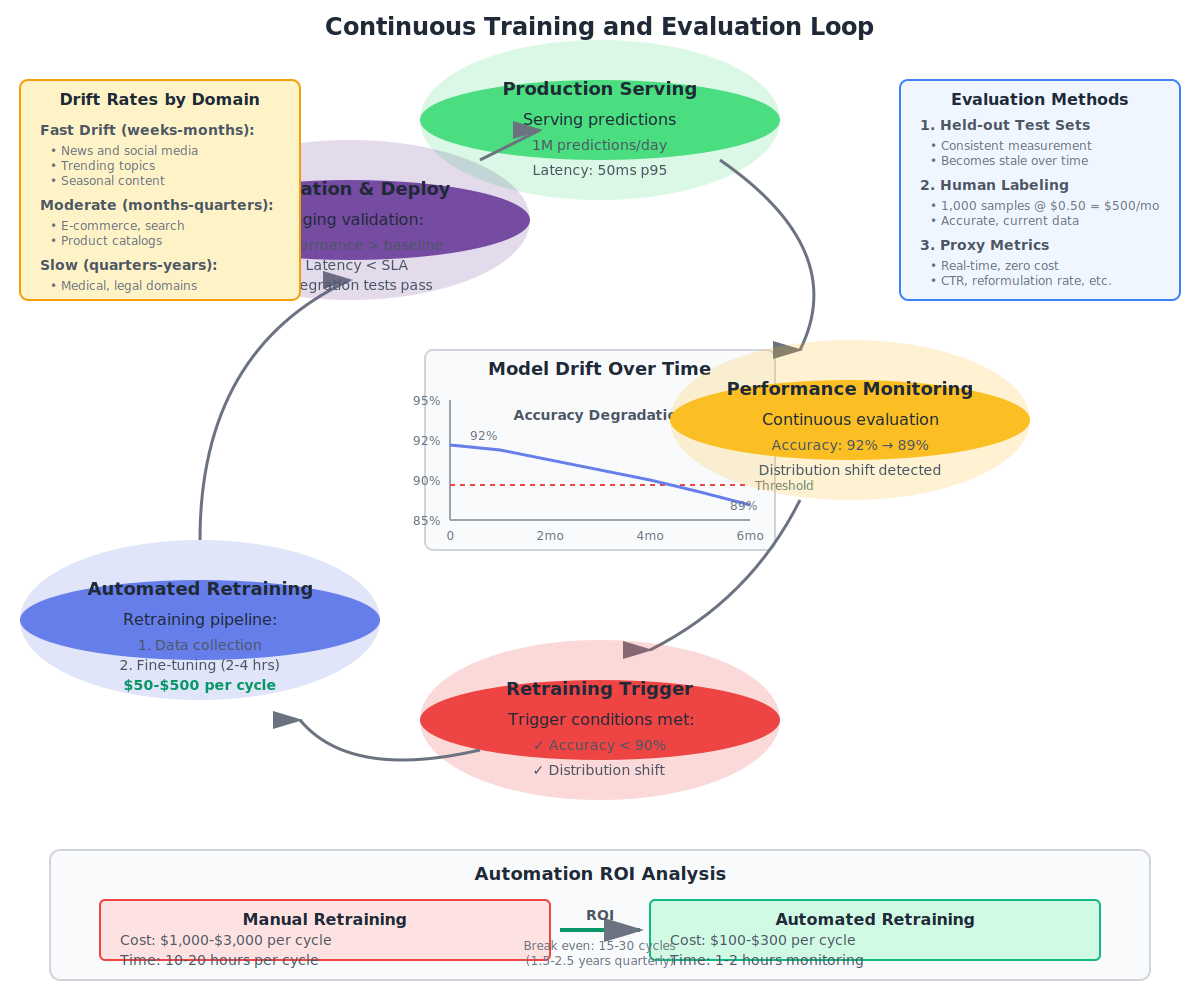
\includegraphics[width=0.95\textwidth]{chapters/diagrams/chapter09_continuous_training_u5v6w7x8.png}
\caption{Continuous training and evaluation loop showing the complete cycle from production serving through performance monitoring, drift detection, automated retraining, and validation. The center graph illustrates model drift over time, with performance degrading from 92\% to 89\% over six months, triggering retraining when the 90\% threshold is crossed.}
\label{fig:continuous_training}
\end{figure}

\subsection{Automation ROI}

Automating the retraining pipeline—data collection, preprocessing, training, evaluation, and deployment—requires upfront engineering investment but provides ongoing operational cost savings. Building a fully automated retraining pipeline typically requires 2-4 engineer-months of effort, costing \$40,000-\$100,000 in engineering time. This investment pays off when retraining frequency and manual effort justify automation.

Manual retraining requires data scientist time for each cycle: collecting and preprocessing data (4-8 hours), configuring and launching training (2-4 hours), evaluating results (2-4 hours), and coordinating deployment (2-4 hours), totaling 10-20 hours per retraining cycle. At \$100-\$150 per hour for data scientist time, manual retraining costs \$1,000-\$3,000 per cycle. Retraining quarterly costs \$4,000-\$12,000 annually; retraining monthly costs \$12,000-\$36,000 annually.

Automated retraining reduces per-cycle costs to infrastructure and monitoring time. After initial automation investment, each retraining cycle requires only monitoring and validation time (1-2 hours), costing \$100-\$300 per cycle. The automation investment breaks even after 15-30 retraining cycles, or 1.5-2.5 years for quarterly retraining, 1-2 years for monthly retraining. For models requiring frequent retraining or organizations managing multiple production models, automation provides clear ROI.

\section{Security and Privacy}

Production AI systems face security threats and privacy requirements distinct from traditional software systems. Model theft, adversarial attacks, data poisoning, and privacy violations represent real risks with significant business and legal consequences. Understanding these threats and implementing appropriate defenses is essential for responsible production deployment.

\subsection{Attack Surface and Threats}

AI systems present multiple attack surfaces. Model theft through API access represents a significant threat: attackers can query a production model repeatedly, collect input-output pairs, and train a substitute model that replicates the original's behavior. For a model serving 1,000 requests per second, an attacker making 10 queries per second for 24 hours collects 864,000 input-output pairs, potentially sufficient to train a substitute model. Rate limiting, query monitoring, and watermarking provide partial defenses, but determined attackers with sufficient resources can often extract substantial model functionality.

Adversarial attacks craft inputs designed to cause model failures. For image classifiers, adversarial examples—images with imperceptible perturbations—can cause misclassification with high confidence. For text models, adversarial prompts can elicit inappropriate responses or leak training data. For recommendation systems, adversarial user behavior can manipulate recommendations. Defending against adversarial attacks requires adversarial training, input validation, and output filtering, adding 10-30\% to training costs and 5-15\% to inference latency.

Data poisoning attacks inject malicious examples into training data, causing models to learn attacker-desired behaviors. For models trained on user-generated content, attackers can create accounts and submit poisoned examples. For models trained on web-scraped data, attackers can publish poisoned content. Defending against data poisoning requires data validation, anomaly detection, and robust training procedures, adding 20-50\% to data preprocessing costs.

Privacy violations occur when models leak training data or enable inference about training examples. Models can memorize specific training examples, particularly rare or unusual ones, and reproduce them in responses. For models trained on sensitive data—medical records, financial information, personal communications—this leakage violates privacy regulations and creates legal liability. Differential privacy and federated learning provide technical defenses, but impose accuracy costs and implementation complexity.

\subsection{Security Techniques}

Rate limiting restricts the number of queries per user or API key, mitigating model theft and denial-of-service attacks. Typical rate limits range from 10-1,000 queries per minute depending on use case and user tier. Implementing rate limiting requires API gateway infrastructure and user authentication, adding \$500-\$2,000 monthly in infrastructure costs for systems serving millions of requests daily.

Query monitoring detects suspicious access patterns indicating potential attacks. Monitoring systems track query frequency, query similarity, error rates, and response patterns. Anomalous patterns—such as a single user making thousands of similar queries, or queries systematically exploring input space—trigger alerts or automatic blocking. Implementing comprehensive monitoring requires logging infrastructure, analysis pipelines, and alerting systems, costing \$2,000-\$10,000 monthly depending on query volume and analysis sophistication.

Model watermarking embeds detectable signatures in model outputs, enabling detection of stolen models. Watermarking techniques modify model behavior on specific trigger inputs, causing watermarked models to produce distinctive outputs. If a competitor's model produces the same distinctive outputs, this provides evidence of model theft. Watermarking adds minimal inference cost but requires careful implementation to avoid degrading model performance on normal inputs.

Adversarial training incorporates adversarial examples into training data, improving model robustness. Training on both normal and adversarial examples teaches models to handle perturbations and edge cases. Adversarial training typically increases training time by 20-50\% and training data requirements by 10-30\%, but significantly improves robustness. For BERT-base, adversarial training might increase training cost from \$1,000 to \$1,200-\$1,500.

\subsection{Privacy Techniques}

Differential privacy provides mathematical guarantees that model training does not leak information about individual training examples. Differential privacy adds calibrated noise during training, ensuring that model parameters do not depend too strongly on any single training example. This prevents memorization of sensitive data and provides formal privacy guarantees. However, differential privacy imposes accuracy costs: typical implementations reduce accuracy by 1-5 percentage points. For a model achieving 92\% accuracy without differential privacy, differentially private training might achieve 87-91\% accuracy.

Implementing differential privacy requires specialized training procedures and careful privacy budget management. Privacy budget—measured in epsilon—quantifies the privacy guarantee: smaller epsilon provides stronger privacy but larger accuracy costs. Typical values range from epsilon=1 (strong privacy, significant accuracy cost) to epsilon=10 (weaker privacy, minimal accuracy cost). Training with differential privacy increases training time by 20-40\% due to additional noise injection and gradient clipping operations.

Federated learning trains models on distributed data without centralizing the data. Instead of collecting data from edge devices or partner organizations, federated learning sends model updates to the data, trains locally, and aggregates only model parameter updates. This approach enables training on sensitive data that cannot be centralized due to privacy regulations or competitive concerns. Federated learning requires coordination infrastructure, secure aggregation protocols, and handling of heterogeneous data distributions, increasing training complexity and cost by 2-5×.

\begin{figure}[htbp]
\centering
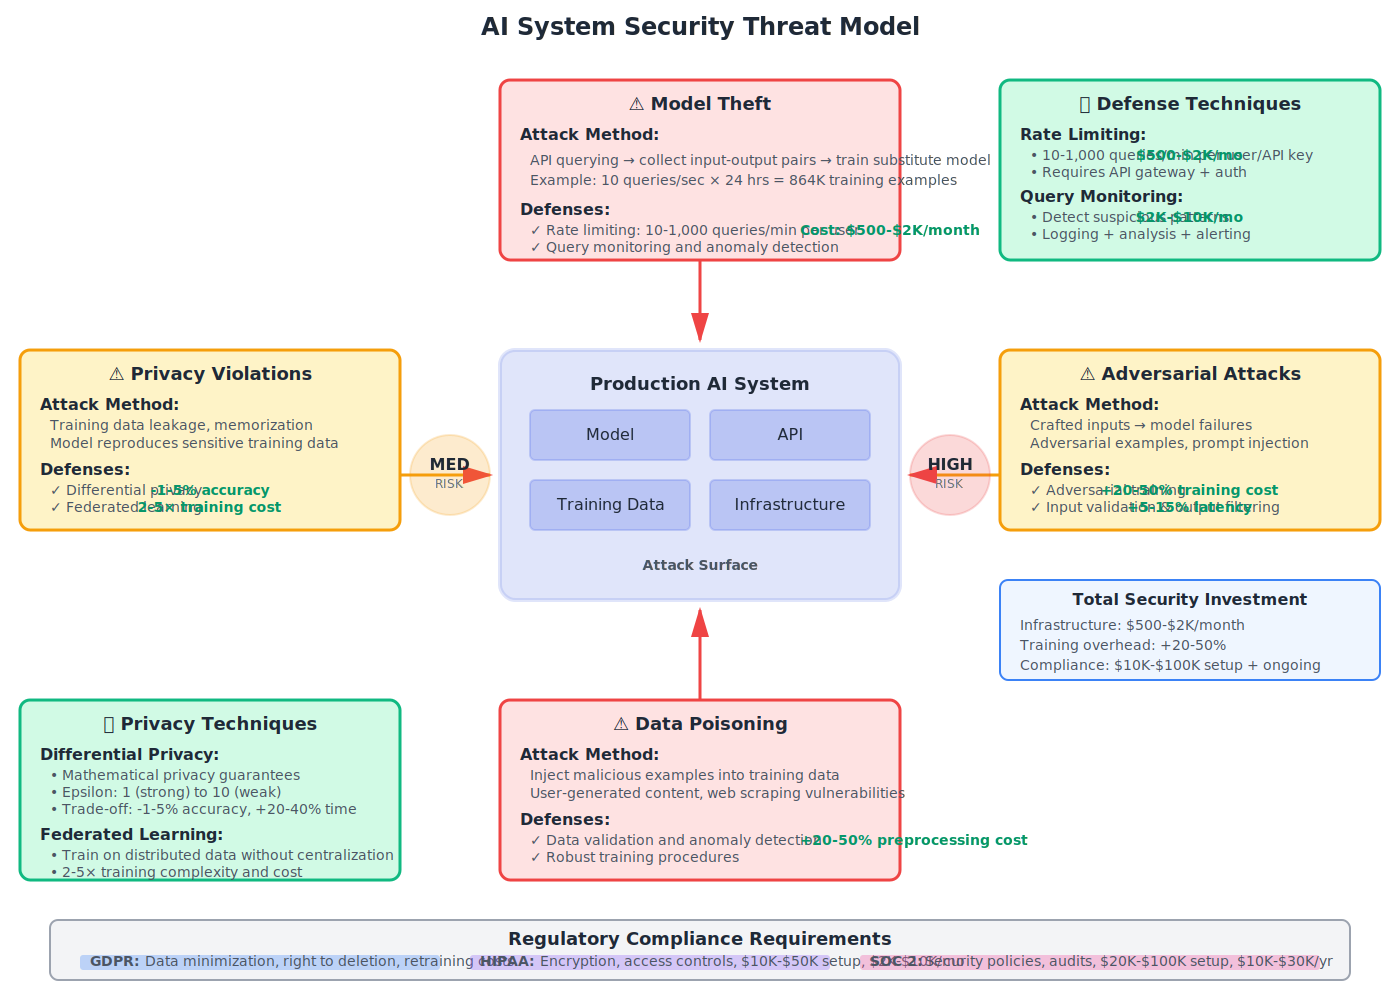
\includegraphics[width=0.95\textwidth]{chapters/diagrams/chapter09_security_threats_y9z0a1b2.png}
\caption{AI system security threat model showing four primary attack vectors: model theft through API querying, adversarial attacks with crafted inputs, data poisoning during training, and privacy violations through data leakage. Each threat includes attack methods, impacts, defense mechanisms, and associated costs. Regulatory compliance requirements (GDPR, HIPAA, SOC 2) are shown at the bottom.}
\label{fig:security_threats}
\end{figure}

\subsection{Compliance Requirements}

Regulatory compliance—GDPR in Europe, HIPAA for healthcare, SOC 2 for enterprise software—imposes specific technical and operational requirements. GDPR requires data minimization, purpose limitation, and the right to deletion. For AI systems, this means training only on necessary data, documenting data usage, and implementing mechanisms to remove individual data points from trained models. Model retraining after data deletion requests can cost \$1,000-\$100,000 depending on model size and retraining frequency.

HIPAA compliance for healthcare AI requires encryption of data at rest and in transit, access controls and audit logging, business associate agreements with vendors, and regular security assessments. Implementing HIPAA-compliant infrastructure typically costs \$10,000-\$50,000 in initial setup and \$2,000-\$10,000 monthly in ongoing compliance costs. These costs include encrypted storage, secure API gateways, audit logging infrastructure, and compliance monitoring.

SOC 2 compliance for enterprise software requires documented security policies, access controls, change management procedures, incident response plans, and annual audits. Achieving SOC 2 certification typically costs \$20,000-\$100,000 in initial implementation and \$10,000-\$30,000 annually for ongoing audits and compliance maintenance. For AI systems, SOC 2 compliance extends to model training, deployment, and monitoring processes.

\section{Cost Optimization Strategies}

Production AI costs typically break down as 40\% training, 50\% inference, and 10\% storage and operations. Understanding this breakdown and implementing targeted optimization strategies can reduce total costs by 30-70\% while maintaining performance and reliability.

\subsection{Training Cost Optimization}

Spot instances reduce training costs by 60-80\% compared to on-demand instances, but introduce interruption risk. Cloud providers offer unused capacity at steep discounts: AWS spot instances for p3.8xlarge (4× V100 GPUs) cost \$3.06 per hour versus \$12.24 on-demand. For training jobs requiring 100 GPU-hours, spot instances cost \$306 versus \$1,224 on-demand, saving \$918 (75\%). However, spot instances can be interrupted with 2-minute warning when capacity is needed elsewhere.

Handling spot interruptions requires checkpointing and automatic restart capabilities. Training code should save checkpoints every 10-30 minutes, enabling restart from the most recent checkpoint after interruption. Implementing robust checkpointing adds 5-10\% training time overhead but enables spot instance usage. For training jobs longer than 4-8 hours, spot instance savings exceed checkpointing overhead, providing net cost reduction.

Mixed precision training reduces training time and memory usage by 40-60\% with minimal accuracy impact. Training in FP16 instead of FP32 halves memory requirements and doubles throughput on modern GPUs with tensor cores. For BERT-base, mixed precision training reduces training time from 20 GPU-hours to 12 GPU-hours, saving \$20-\$40 per training run. Implementing mixed precision requires framework support (PyTorch AMP, TensorFlow mixed precision) and careful loss scaling to prevent numerical instability.

Gradient accumulation enables training with larger effective batch sizes on limited hardware. Instead of processing a 512-example batch in one step, gradient accumulation processes 8 batches of 64 examples, accumulating gradients before updating parameters. This technique enables training large models on smaller GPUs, avoiding the need for expensive multi-GPU setups. For models requiring 32 GB memory with batch size 512, gradient accumulation enables training on 16 GB GPUs, reducing hardware costs from \$2.50 per hour (A100 40GB) to \$1.20 per hour (A10G 24GB).

\subsection{Inference Cost Optimization}

Model compression reduces inference costs by 50-90\% through quantization, pruning, and distillation. Quantization converts FP32 weights to INT8, reducing model size by 75\% and increasing throughput by 2-4×. For BERT-base, quantization reduces model size from 440 MB to 110 MB and increases throughput from 100 to 300 sequences per second on CPU. This enables serving the same traffic with one-third the infrastructure, reducing costs from \$15,000 to \$5,000 monthly.

Pruning removes unnecessary model parameters, reducing model size and computation. Structured pruning removes entire attention heads or feed-forward layers, while unstructured pruning removes individual weights. Typical pruning removes 30-50\% of parameters with 1-2\% accuracy loss. For BERT-base, pruning 40\% of parameters reduces inference time by 30-40\%, enabling similar cost savings as quantization.

Knowledge distillation trains smaller student models to mimic larger teacher models, achieving 90-95\% of teacher performance with 50-90\% fewer parameters. Distilling BERT-base (110M parameters) to DistilBERT (66M parameters) maintains 97\% of performance while reducing inference cost by 60\%. Distillation requires additional training cost—typically 20-50\% of original training cost—but provides ongoing inference savings that quickly exceed the upfront investment.

Caching reduces redundant computation for repeated queries. For search systems, recommendation systems, and content moderation, many queries repeat or are similar. Caching results for common queries eliminates redundant inference. A cache with 10\% hit rate reduces inference costs by 10\%; a cache with 50\% hit rate reduces costs by 50\%. Implementing caching requires cache infrastructure (Redis, Memcached) costing \$500-\$2,000 monthly, but saves \$5,000-\$50,000 monthly in inference costs for high-traffic systems.

Batching aggregates multiple requests for parallel processing, increasing throughput by 5-20×. Processing requests individually achieves 10-20 sequences per second on GPU; batching 32 requests achieves 200-400 sequences per second. Batching requires request queuing and introduces latency—typically 10-50ms additional latency depending on batch size and arrival rate. For systems with relaxed latency requirements (100-500ms acceptable), batching provides substantial cost savings.

\subsection{Infrastructure Optimization}

Right-sizing instances matches infrastructure capacity to actual requirements, eliminating waste. Many production systems over-provision infrastructure for peak load, resulting in 30-60\% average utilization. Monitoring actual resource usage and adjusting instance types and counts can reduce costs by 20-40\%. For a system using 8× g4dn.xlarge instances (4 GPUs, 16 GB memory each) at 40\% average utilization, right-sizing to 4× g4dn.2xlarge instances (8 GPUs, 32 GB memory each) at 80\% utilization reduces costs from \$6,144 to \$4,608 monthly, saving \$1,536 (25\%).

Auto-scaling adjusts capacity based on traffic patterns, reducing costs during low-traffic periods. For systems with predictable daily or weekly patterns—such as business applications with low weekend traffic—auto-scaling can reduce average capacity by 20-40\%. Implementing auto-scaling requires load balancing, health checks, and scaling policies, adding \$500-\$1,000 monthly in infrastructure complexity, but saving \$5,000-\$20,000 monthly for systems with significant traffic variation.

Reserved instances and savings plans reduce costs by 30-50\% for predictable baseline capacity. Committing to one-year or three-year reserved capacity provides substantial discounts: AWS p3.8xlarge on-demand costs \$12.24 per hour; one-year reserved costs \$7.54 per hour (38\% savings); three-year reserved costs \$4.89 per hour (60\% savings). For production systems with stable baseline load, reserved instances for baseline capacity combined with on-demand or spot instances for peak capacity optimizes costs.

\subsection{Monitoring and Attribution}

Cost monitoring and attribution enables identification of optimization opportunities and budget accountability. Comprehensive cost tracking requires tagging resources by project, team, environment, and model version, enabling analysis of cost drivers and trends. Cloud provider cost management tools (AWS Cost Explorer, GCP Cost Management, Azure Cost Management) provide basic tracking, but detailed attribution requires custom tagging and analysis.

Key cost metrics include cost per prediction, cost per user, cost per model version, training cost per experiment, and infrastructure cost by component. Tracking these metrics over time reveals trends and anomalies. For example, cost per prediction increasing from \$0.001 to \$0.003 indicates efficiency degradation requiring investigation. Training cost per experiment increasing from \$500 to \$2,000 suggests scope creep or inefficient experimentation.

Budget planning requires forecasting costs based on traffic growth, model complexity evolution, and retraining frequency. A production system serving 1 million predictions daily at \$0.001 per prediction costs \$30,000 monthly. Projecting 50\% annual traffic growth and 20\% efficiency improvement yields \$33,750 monthly cost in year two (\$30,000 × 1.5 ÷ 1.2). Adding quarterly retraining at \$5,000 per cycle adds \$1,667 monthly (\$5,000 × 4 ÷ 12), totaling \$35,417 monthly or \$425,000 annually.

\begin{figure}[htbp]
\centering
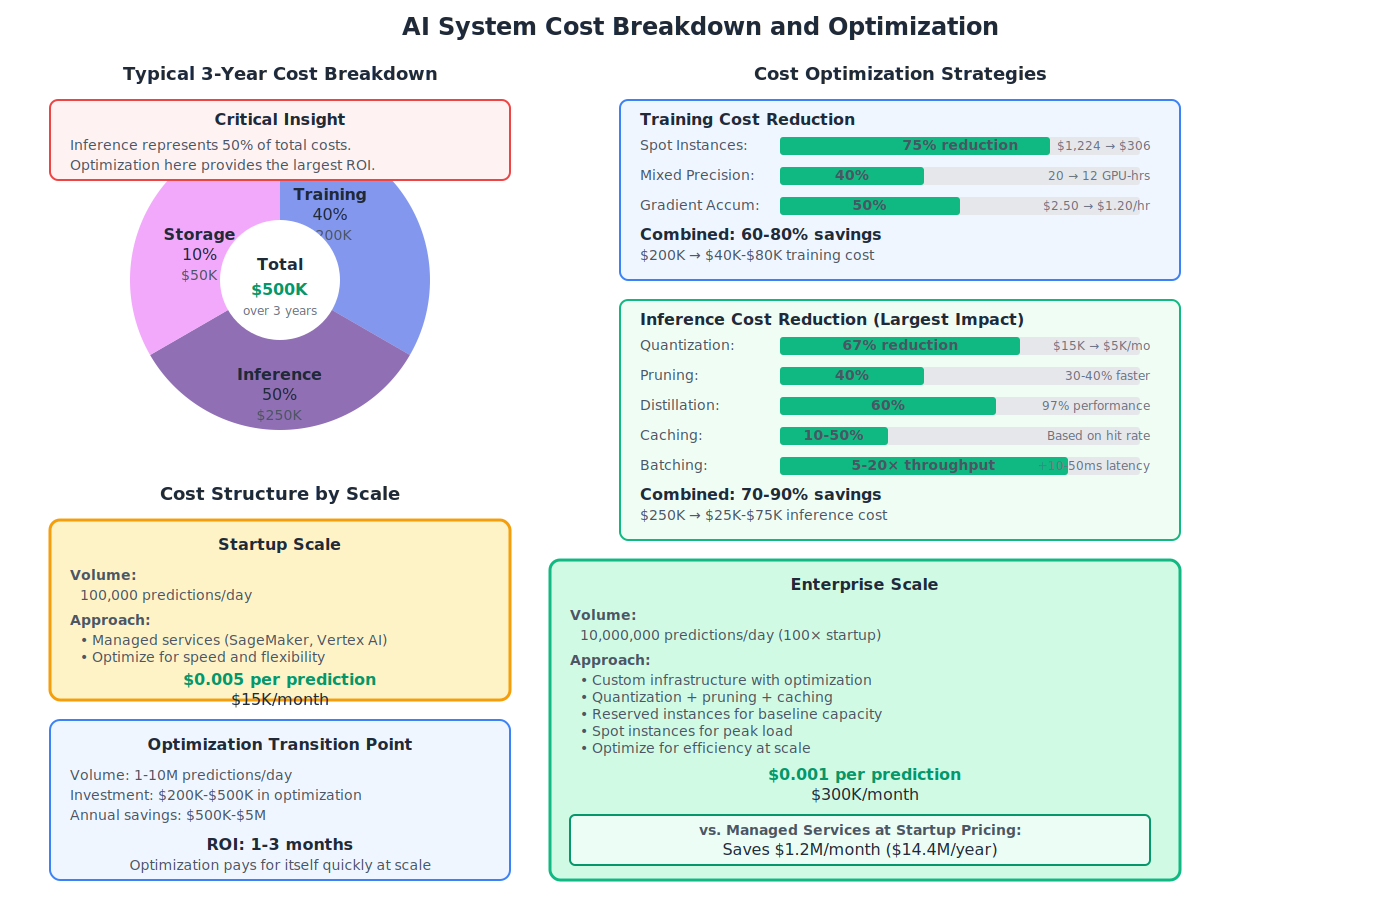
\includegraphics[width=0.95\textwidth]{chapters/diagrams/chapter09_cost_breakdown_c3d4e5f6.png}
\caption{AI system cost breakdown and optimization strategies showing typical three-year costs (40\% training, 50\% inference, 10\% storage/ops) and specific optimization techniques with quantified savings. Training optimizations (spot instances, mixed precision, gradient accumulation) provide 60-80\% savings. Inference optimizations (quantization, pruning, distillation, caching, batching) provide 70-90\% savings. The scale comparison shows the transition point where custom optimization becomes economically justified.}
\label{fig:cost_breakdown}
\end{figure}

\subsection{Startup versus Enterprise Costs}

Cost structures differ significantly between startups and enterprises. Startups typically optimize for speed and flexibility, accepting higher per-unit costs to minimize upfront investment and maintain agility. Enterprises optimize for efficiency and reliability, investing in infrastructure and automation to reduce long-term costs.

A startup serving 100,000 predictions daily might use managed services (AWS SageMaker, Google Vertex AI) at \$0.005 per prediction, costing \$15,000 monthly. This approach requires minimal engineering effort and provides instant scalability, but costs 5× more per prediction than optimized infrastructure. For early-stage startups, this trade-off makes sense: \$15,000 monthly in infrastructure costs is manageable, while the engineering effort to optimize costs (2-3 engineer-months, \$40,000-\$75,000) exceeds short-term savings.

An enterprise serving 10 million predictions daily faces different economics. At \$0.005 per prediction, costs reach \$1.5 million monthly—\$18 million annually. Investing \$200,000-\$500,000 in infrastructure optimization to reduce per-prediction costs to \$0.001 saves \$1.2 million monthly—\$14.4 million annually—providing immediate ROI. Enterprise scale justifies dedicated infrastructure, custom optimization, and operational automation.

\section*{Key Insights}

\textbf{Operational Costs Dominate Total Cost of Ownership}: Training represents 20-30\% of three-year costs; inference and operations represent 70-80\%. A model costing \$50,000 to train typically costs \$150,000-\$400,000 annually to operate. Budget planning must account for ongoing operational costs, not just initial training investment. Organizations underestimating operational costs face budget overruns and sustainability challenges.

\textbf{Model Drift Requires Systematic Retraining}: Model performance degrades over time as production data distributions shift. Degradation rates vary by domain: news and social media drift rapidly (weeks to months), e-commerce moderately (months to quarters), medical and legal slowly (quarters to years). Retraining frequency should be driven by measured performance degradation and distribution shift, not arbitrary schedules. Fine-tuning from previous versions reduces retraining costs by 80-90\% compared to training from scratch.

\textbf{Automation Provides Clear ROI at Scale}: Building automated retraining pipelines requires \$40,000-\$100,000 upfront investment but reduces per-cycle costs from \$1,000-\$3,000 to \$100-\$300. Automation breaks even after 15-30 retraining cycles, or 1.5-2.5 years for quarterly retraining. For models requiring frequent retraining or organizations managing multiple production models, automation is essential for sustainable operations.

\textbf{Security and Privacy Impose Real Costs}: Implementing differential privacy reduces accuracy by 1-5 percentage points and increases training time by 20-40\%. Adversarial training increases training costs by 20-50\%. Regulatory compliance (HIPAA, SOC 2) adds \$10,000-\$50,000 in initial setup and \$2,000-\$10,000 monthly in ongoing costs. These costs are necessary for responsible deployment and regulatory compliance, but must be factored into project budgets and ROI calculations.

\textbf{Inference Optimization Provides Largest Cost Savings}: Inference typically represents 50\% of total costs. Model compression (quantization, pruning, distillation) reduces inference costs by 50-90\% with minimal accuracy impact. Caching reduces costs by 10-50\% for systems with repeated queries. Batching increases throughput by 5-20×. Combined, these optimizations can reduce inference costs by 70-90\%, providing \$50,000-\$500,000 annual savings for production systems.

\textbf{Cost Structure Differs by Scale}: Startups optimize for speed and flexibility, accepting \$0.003-\$0.005 per prediction using managed services. Enterprises optimize for efficiency, investing in infrastructure to achieve \$0.0005-\$0.001 per prediction. The transition point occurs around 1-10 million predictions daily, where optimization investment (\$200,000-\$500,000) provides clear ROI through ongoing savings (\$500,000-\$5,000,000 annually).

\textbf{Comprehensive Monitoring Enables Optimization}: Cost monitoring and attribution—tracking cost per prediction, cost per user, cost per model version—reveals optimization opportunities and ensures budget accountability. Without detailed monitoring, cost drivers remain opaque and optimization efforts lack focus. Implementing comprehensive monitoring requires custom tagging and analysis but provides essential visibility for cost management.
